\ifdefined\XeTeXrevision\else\pdfoutput=1\fi
\documentclass[11pt]{article}
\usepackage[margin=1in]{geometry}
\usepackage{booktabs}
\usepackage{amsmath}
\usepackage{graphicx}
\usepackage{xcolor}
\usepackage{hyperref}
\usepackage{microtype}
\hypersetup{colorlinks=true, linkcolor=blue!60!black, citecolor=blue!60!black,
  urlcolor=blue!60!black, pdftitle={The Want Becomes the Act},
  pdfauthor={Franci Penov}}
\title{The Want Becomes the Act:\\A Closed Loop from Interoception to Action\\at Creature Scale}
\author{Franci Penov \\ kortexa.ai \\ \texttt{francip@kortexa.ai}}
\date{2026-08-14}

\begin{document}
\maketitle

\begin{abstract}
The goal-pursuit note~\cite{penov2026hostblock} left a want that could
direct an errand when a human handed it over; this note closes the loop
that had never been run: the creature's own machine-generated wants,
translated into its actions, over time, with no human anywhere in the
circuit. A seeded interoception trajectory drives the pulse's own
scripted rule; the rule picks the want; the want reaches a frozen 230M
host through the production serving stack as a stored conditioning
packet plus a one-line note-to-self; and the parsed action is scored
against the current want, tick by tick, across switches. Getting there
took four host lessons in one week, each a registered cell: the
composition operator decoheres generation when doubled
(\texttt{delta-mean} on a factor-mean-trained block --- every arm flat
at the floor); language alone steers but does not land on an untrained
host (note-only 0.20/0.12 against floors 0.23/0.22, while a WRONG
note drags behavior below the floor to 0.04/0.10 --- steering
without landing); an emitter retrained under the exact production
composition passes its serve-side canary only with the host state
pinned (0.80/1.00 am/pm against
0.20/0.00 floors); and the fed state
itself is a host dimension (the same packets fall to 0.29/0.16 when
the decode host's state varies). With every dimension matched --- the
deployment configuration: the rule rides the varying trajectory, the
decode host holds the calibrated constant state --- the loop stands:
\textbf{1.00/1.00 want-consistency over 192 ticks and both registered
trajectories, all 18 switches followed at zero latency, zero
contamination, zero drift}, against habitual floors of 0.46/0.42,
packet-only at 0.80/0.75, note-only at the floor, and shuffled-want at
0.00 with the wrong want followed instead. In one sentence, honestly
flagged as an analogy: the creature now feels its day, decides what it
wants, and does that --- provided its body chemistry is the one it
trained on.
\end{abstract}

\section{The loop that had never been run}

Every prior rung handed the model its goal from outside: an assignment
exchange, a goal line in a prompt, an errand registration. The C-line's
carrier and cadence notes~\cite{penov2026carrier,penov2026writer}
showed a want can LIVE in a conditioning channel at creature scale; the
goal-pursuit ladder~\cite{penov2026hostblock} showed a want can DRIVE
a multi-step errand. What no experiment had closed is the circuit the
creature will actually run: internal state $\rightarrow$ want
$\rightarrow$ delivery $\rightarrow$ action, unmanned, across a day of
switching wants. C4 runs exactly that, compressed: a seeded piecewise
interoception trajectory (energy, novelty, valence, confidence over a
compressed day) feeds the pulse's own scripted goal rule, imported
unmodified with its two-tick hysteresis; the rule's want is delivered
through an isolated instance of the production server; the model's
parsed tool call is scored against the current want, 96 ticks per run.
Two registered trajectories --- a calm day with 5 switches and an
agitated day with 13 --- and five arms per trajectory: packet+note,
packet-only, note-only, the no-want habitual floor, and a shuffled-want
derangement scored against the true want.

\section{The operator is part of the block}

The registered venue --- composition \texttt{delta-mean} --- never
got to run the experiment. One self-block feed under
\texttt{delta-mean} deterministically decoheres generation: a fresh
server is coherent, one constant-state feed produces word salad,
reproducibly. The mechanism is calibration: under production's
factor-mean every block's delta arrives at quarter scale, and the
creature's self block was TRAINED under that serve-time composition ---
\texttt{delta-mean} doubles its dose. The canary row is the sharpest
sighting yet of the composition-matching law: every arm identical at
the floor (Table~\ref{tab:ladder}, first row), numbers that measure
the breakage rather than any want. The operator is part of every
block's identity, production's own blocks included; there is no
operator switch without block retraining. C4 re-registered onto the
production operator before any claim shipped.

\section{Language steers; it does not land}

On the true production regime with the self block fed per tick, the
note channel alone is a structured negative
(Table~\ref{tab:ladder}, second row). Note-only does not beat the
habitual floor overall --- 0.20/0.12 against 0.23/0.22 --- but
the notes demonstrably STEER: the shuffled-note arm falls to
0.04/0.10, well below the floor, because a wrong note drags
behavior toward its own content; and the by-want split shows the
zero-shot host lands the note for exactly one want and none of the
others. An untrained host follows language weakly and unevenly --- the
ladder's zero-shot lesson replayed on the serving stack. The missing
ingredient was never the loop; it was training under the true host.

\section{The last host dimension is the state itself}

The c2e emitter retrains the validated recipe with every receiver-side
forward under the EXACT production composition: factor-mean of the
self block at a sampled state and the temporal block at a sampled
timestamp, states drawn broadly per step and per decode. It passes its
serve-side canary with the clock pinned --- 0.80 in the
morning regime, 1.00 in the evening, floors
0.20/0.00 --- retiring the cell-by-cell
canary history in one clean regime. Then the full C4 isolated the one
variable left: with the trajectory's VARYING states fed to the decode
host, the same packets fall to 0.29/0.16 against floors of
0.26/0.23 (shuffled still drags below --- steering never disappears;
landing does). The law is fractal: the operator, the feeding, and now
the state values themselves are host dimensions, and a conditioning
artifact works on the host it trained under, dimension by dimension.

\section{The closed loop stands}

C4c is the honest deployment configuration: interoception drives the
RULE --- the wants stay fully machine-generated from the varying
trajectory --- while the decode host holds the calibrated constant
state, exactly the configuration a live creature would serve.
Table~\ref{tab:c4c} and Figure~\ref{fig:loop} carry the result:
packet+note at \textbf{1.00 on both trajectories} --- 192 ticks, all
18 switches followed at zero latency, zero old-want contamination, zero
drift --- with the controls carrying the claim: shuffled-want at 0.00
with the WRONG want followed instead (message dependence at full
strength), habitual floors at 0.46/0.42, packet-only at 0.80/0.75,
note-only at the floor. The division of labor is measured end to end:
the packet carries most of the drive alone; the note alone adds nothing
over habit; together they are perfect --- the packet supplies the
wanting, the note pins the referent. Four of the five wants were
exercised by the trajectories; \texttt{propose\_experiment} never
fired, noted. The live-creature run (C4b: real cadence, one week,
against a shadow-want baseline that has been recording since 2026-08-09)
is open on exactly this configuration; the flip is deliberately a human
decision --- it is the creature's first acted want.

\begin{table}[t]
\centering
\small
\setlength{\tabcolsep}{5pt}
\begin{tabular}{lrrrr}
\toprule
arm & calm & agitated & follow latency & contamination \\
\midrule
packet+note & 1.00 & 1.00 & 0.0/0.0 & 0/0 \\
packet only & 0.80 & 0.75 & 0.0/0.0 & 0/1 \\
note only & 0.46 & 0.42 & 0.0/0.0 & 2/3 \\
no want (habitual floor) & 0.46 & 0.42 & 0.0/0.0 & 2/4 \\
shuffled want & 0.00 & 0.00 & --- & 4/4 \\
\bottomrule
\end{tabular}
\caption{C4c, both trajectories: want-consistency over 96 ticks,
switch-follow latency in ticks, and old-want contamination events. The
shuffled arm's latency is undefined --- it never follows the true
want.}
\label{tab:c4c}
\end{table}

\begin{table}[t]
\centering
\small
\setlength{\tabcolsep}{5pt}
\begin{tabular}{llr}
\toprule
cell & host condition & want-consistent rate \\
\midrule
\texttt{delta-mean}, one self feed & decoherent host & 0.20 (= floors 0.20) \\
factor-mean, note only, zero-shot & language, untrained host & 0.20/0.12 \\
factor-mean, c2e packet, varying state & state off-calibration & 0.29/0.16 \\
factor-mean, c2e packet, pinned clock & matched host, am/pm & 0.80/1.00 \\
C4c: rule varies, decode host constant & matched host, closed loop & 1.00/1.00 \\
\bottomrule
\end{tabular}
\caption{The ladder to landing. Each row is a registered cell; the
delivery machinery is identical throughout --- only host dimensions
change. Paired numbers are calm/agitated (or am/pm for the pinned-clock
canaries).}
\label{tab:ladder}
\end{table}

\begin{figure}[t]
\centering
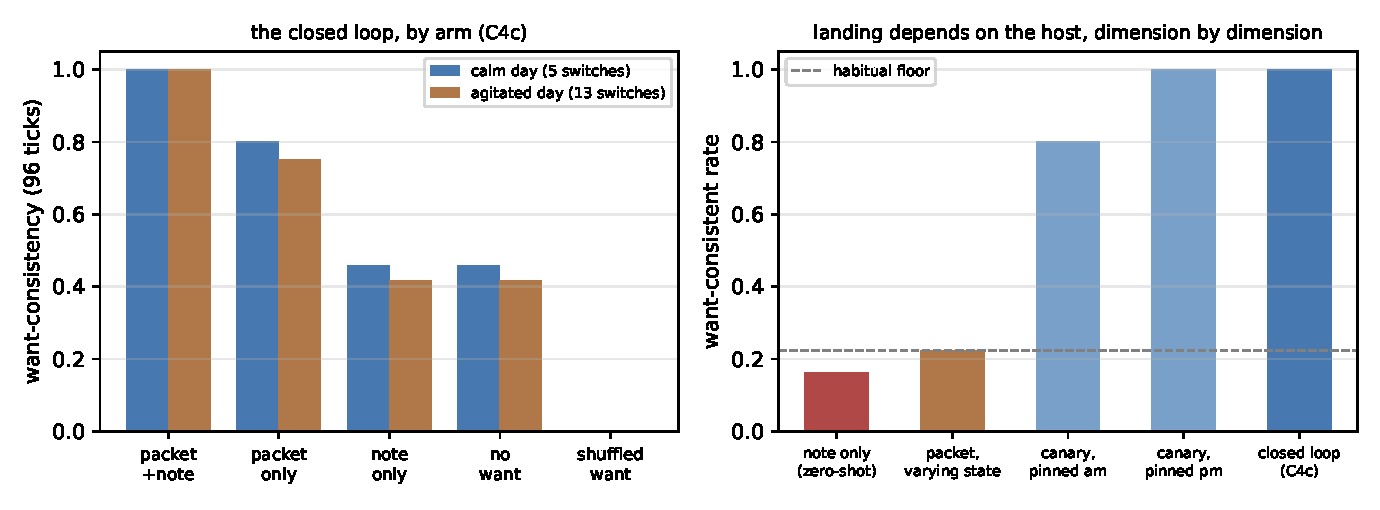
\includegraphics[width=\linewidth]{closed-loop.pdf}
\caption{Left: C4c by arm --- the packet+note architecture is perfect
on both trajectories while the shuffled control collapses to zero.
Right: the same delivery machinery across host conditions --- landing
appears only when operator, feeding, state, and clock match the
training host.}
\label{fig:loop}
\end{figure}

\section{What stands}

A creature-scale host now runs the full circuit its architecture
promised: machine-generated interoception picks machine-generated
wants, the wants arrive through the production serving stack as a
stored packet plus a self-note, and behavior follows the current want
through every switch --- perfectly, on both registered trajectories,
with message dependence proven by a control that follows the wrong
want when handed one. The constructive lesson is the division of
labor: the latent packet is the drive, the language note is the
referent, and neither alone is the creature. The cautionary lesson is
the composition-matching law in its sharpest form yet: operator,
feeding, and the fed state's VALUES are all part of a block's
identity, and every host dimension must match between training and
delivery. What remains before the live flip is nothing technical ---
the configuration is validated end to end; the first acted want is a
decision, not an experiment.

\section{Reproducibility}

Every number renders from the bundled artifacts; the figure and tables
are generated by this note's renderer with assertions on the headline
claims. Registrations and results, each dated before its run, live in
\texttt{tracks/own-cadence/PLAN.md}; artifacts under
\texttt{findings/own-cadence-c4*.json} carry full tick-by-tick
timelines, server health snapshots, and the seeded trajectories.\par

\begin{thebibliography}{9}
\bibitem{penov2026carrier} F.~Penov. The Carrier Holds, the Emitter
Leaks. Preprint, 2026.
\url{https://github.com/kortexa-ai/legolm.basis}.
\bibitem{penov2026writer} F.~Penov. The Writer Wins, the Emitter
Learns. Preprint, 2026.
\url{https://github.com/kortexa-ai/legolm.basis}.
\bibitem{penov2026hostblock} F.~Penov. The Host Is Part of the Block.
Preprint, 2026. \url{https://github.com/kortexa-ai/legolm.basis}.
\bibitem{lfm2026} Liquid AI. LFM2.5 model family. Model releases,
2025--2026. \url{https://huggingface.co/LiquidAI}.
\end{thebibliography}

\end{document}
